% !TEX root = ../thesis-sample.tex

\chapter{Autonomous Exploration in 2D Space} \label{chap:ae2D}

The goal of autonomous exploration is to select robotic actions designed to minimize map uncertainty, thereby maximizing map information gain. We formulate autonomous exploration as an optimization problem to determine a policy that accounts for map uncertainty and travel cost.

\section{Entropy-Based Exploration}

In this section, we define Shannon's entropy as a measure of map uncertainty, and present a novel approach to predict future entropy from an arbitrary ray. Then we discuss computational modifications for real-time implementation.

\subsection{Shannon's Entropy}

Here we present how the probabilistic properties of an occupancy grid map provide key information about the uncertainty of the space for motion planning. Shannon's entropy commonly serves as an uncertainty measure~\cite{StaGriBur05}. Provided grid cell probabilities of map $m$, Shannon's entropy is defined as
\begin{align}
\label{eqn:ShannonsEntropyCell}
H(P(\mathbf{m}_i))&=-P(\mathbf{m}_i)\log{P(\mathbf{m}_i})-P(\bar{\mathbf{m}}_i)\log{P(\bar{\mathbf{m}}_i}),
\\
\label{eqn:ShannonsEntropyMap}
H(P(m))&=\sum_{i=1}^{n_m}H(P(\mathbf{m}_i)),
\end{align}
for an individual cell and the entire map, respectively.
Thus, entropy is maximized when $P(\mathbf{m}_i)=0.5$, which corresponds to the largest uncertainty; similarly, entropy is minimized as $P(\mathbf{m}_i)$ approaches $0$ or $1$, which corresponds to the smallest uncertainty. %; thus Shannon's entropy is a measure of uncertainty.



\subsection{Expected Information Gain}

Suppose a future pose candidate and its associated future measurement scan is $X_c=\braces{x_c,R_c}$ and $Z_c$, respectively, where $c\in\mathcal C$ such that $\mathcal C=\braces{1,2,...,n_c}$ accounts for all $n_c$ candidates under consideration for the next robot pose. The current pose of the robot is \emph{not} $X_c$ in general, so any change to the probabilistic map from $X_c$ must be predicted. Much like the probabilistic mapping, this is achieved ray-by-ray~\cite{KauAiLee16,KauTakAiLee17}. Considering that all grid cell probabilities are conditioned on the history of poses $X_{1:t}$ and measurement scans $Z_{1:t}$, these terms are removed from the remaining equations for simplicity. 

\begin{prop}
\label{prop:ExpectedH}
For candidate ray $z_c$, the expected entropy is
\begin{align}
\label{eqn:DiscExpEntropyRay}
&\text{E}[H(P(m|x_c,z_{c}))]=\sum_{k=1}^{n_{r}+1}\bigg\{H(P(m|x_c,z_{c,k}))P(z_{c,k}|x_c)\bigg\},
\end{align}
where $z_{c,k}$ refers to the distance from $x_c$ to the $k$-th grid cell along the measurement ray. The first term of the summation of \refeqn{DiscExpEntropyRay}, namely $H(P(m|x_c,z_{c,k}))$, is obtained with entropy definitions \refeqn{ShannonsEntropyCell}, \refeqn{ShannonsEntropyMap} and the inverse sensor model \refeqn{RayISMAnswer}--\refeqn{Unnormalized}. The second term is derived from \refeqn{allEta} with
\begin{align}
\label{eqn:ProbMeas}
P(z_{c,k}|x_c)&=\frac{p(z_{c,k}|x_c)}{\sum_{i=1}^{n_{r}+1}p(z_{c,i}|x_c)}=\frac{\eta_{c,k}^{-1}}{\sum_{i=1}^{n_{r}+1}\eta_{c,i}^{-1}},
\end{align}
where $\eta_{c,k}$ refers to the normalizer based on the measurement $z_{c,k}$.
The expected negative entropy change for candidate pose $X_c$ is equivalently the expected information gain from ray $z_c$,
\begin{align}
\label{eqn:expectedInfoGainRay}
\mathcal I(X_c,z_c)&=H(P(m))-\text{E}\left[H(P(m|X_c,z_c))\right].
\end{align}
\end{prop}
\begin{proof}% TODO: add ref?
See Appendix B.
\end{proof}

The proposed approach discretizes the measurement according to assumptions of occupancy grid mapping, and exploits the probabilistic properties uncovered by the proposed inverse sensor model. These are used to directly calculate the expected value of map entropy for a single measurement ray. 





\subsection{Computational Limitations and Approximations}

The computational order for each measurement ray is $\mathcal O(n_{r}^2)$ since the summations of \refeqn{ProbMeas} are embedded in \refeqn{DiscExpEntropyRay}. However, several of those intersections provide negligible information since the probability of the measurement ray capturing certain cell depths is close to zero.

The approximation of expected ray entropy provides a method to reduce the computation of \refeqn{expectedInfoGainRay} substantially. This goal is achieved by systematically selecting a smaller set of grid cells to consider over the summations of \refeqn{DiscExpEntropyRay} and \refeqn{ProbMeas}.
The smaller set is determined by the probability that each cell is captured by the measurement ray, known as the detection probability. This can be found recursively as
\begin{align}
\label{eqn:ProbOfFirstCell}
P(\mathbf{r}_{k+})%\nonumber\\&
=\bigg\{\prod_{j=0}^{k-1}P(\bar{\mathbf{r}}_{j})\bigg\}P(\mathbf{r}_{k}),
\end{align}
which is the probability that $\mathbf{r}_{k}$ is the closest occupied grid cell based on past poses and measurement scans, independent of cells beyond the $k$-th cell from $x_c$.
Let $\hat n>0$ be a fixed number of grid cells for all rays such that $\hat n\leq n_{r}+1$ for all $l$.
Let $\hat{r}$ correspond to the grid cells that yield the $\hat{n}$ maximum values of \refeqn{ProbOfFirstCell} (the $\hat n$ most likely ray detections), indexed by increasing distance from candidate location $x_c$.
By replacing the reduced map $r$ with $\hat{r}$ and changing the summation limits to $\braces{1,2,...,\hat n}$ in \refeqn{DiscExpEntropyRay} and \refeqn{ProbMeas}, the order of computation is reduced to $\mathcal O({\hat{n}}^2)$.
Even though the value of $n_{r}$ is different among various rays in general, $\hat n$ is fixed, so the computational order is fixed as well.
In short, this method reduces the required computation substantially by systematically neglecting those grid cells with little effect. It can be noted that if $\hat n=n_{r}+1$, the ray objective function is computed without approximation.


\paragraph{Algorithm} We present an algorithm pseudocode providing the necessary steps to obtain the objective function for a single measurement ray (Algorithm \ref{alg:RayExpectedEntropyGain}). Much like the algorithm pseudocode for the ray-by-ray inverse sensor model (Algorithm \ref{alg:RayByRayISM}), the variable $a_\text{temp}$ serves as an intermediate variable designed to avoid repeated calculations.
Since this algorithm operates as a function, fixed indices and condition variables are removed for simplification. 

\vspace*{0.05\columnwidth}
\begin{algorithm}[H]
	Function: $\mathcal I_\text{ray}=\text{RayExpInfoGain}(x,P(r),z_{1:n_{r}})$\;
	Initialize $P(\bar{\mathbf{r}}_{0})=P(\hat{\bar{\mathbf{r}}}_{0})=P(\bar{\mathbf{r}}_{n_{r}+1})=1$\;
	\For{$k = 1,2,\ldots,n_{r}+1$}{
		$P(\mathbf{r}_{k+}) = P(\bar{\mathbf{r}}_{0:k-1})P(\mathbf{r}_{k})$\;
		$P(\bar{\mathbf{r}}_{0:k})=P(\bar{\mathbf{r}}_{0:k-1})(1-P(\mathbf{r}_{k}))$\;
	}
	Find $\hat r\subset r$ of the $\hat n$ greatest values of 
	$\braces{P(\mathbf{r}_{1+}),P(\mathbf{r}_{2+}),\ldots,P(\mathbf{r}_{(n_{r}+1)+})}$\;
	\For{$k = 1,2,\ldots,\hat{n}$}{
		$P(\hat{\mathbf{r}}_{k+}) = P(\hat{\bar{\mathbf{r}}}_{0:k-1})P(\hat{\mathbf{r}}_{k})$\;
		$P(\hat{\bar{\mathbf{r}}}_{0:k})=P(\hat{\bar{\mathbf{r}}}_{0:k-1})P(\hat{\bar{\mathbf{r}}}_{k})$\;
	}
	\For{$k_\text{m}=1,2,\ldots,\hat n$}{
		Initialize $\eta^{-1}_{k_\text{m}}=0$\;
		\For{$k_\text{c}=1,2,\ldots,\hat n$}{
			$a_\text{temp}=P(\hat{\mathbf{r}}_{k_\text{c}+})p(z_{k_\text{m}}|\hat{\mathbf{r}}_{k_\text{c}+},x)$\;
			$\tilde P(\hat{\mathbf{r}}_{k_\text{c}}|x,z_{k_\text{m}})=P(\hat{\mathbf{r}}_{k_\text{c}})\eta^{-1}_{k_\text{m}}+a_\text{temp}$\;
			$\eta^{-1}_{k_\text{m}}=\eta^{-1}_{k_\text{m}}+a_\text{temp}$\;
		}
		$P(\hat{\mathbf{r}}_{k_\text{c}}|x,z_{k_\text{m}})=\eta_{k_\text{m}}\tilde P(\hat{\mathbf{r}}_{k_\text{c}}|x,z_{k_\text{m}})$ for all $k_\text{c}=1,2,\ldots,\hat n$\;
	}
	$P(z_{k_\text{m}}|x)=\frac{\eta^{-1}_{k_\text{m}}}{\sum_{i=1}^{\hat n}\eta^{-1}_{i}}$ for $k_\text{m}=1,2,\ldots,\hat n$\;
	Initialize $\mathcal I_\text{ray}=0$\;
	\For{$k_\text{c}=1,2,\ldots,\hat n$}{
		$\mathcal I_\text{ray}=\mathcal I_\text{ray}+H(P(\hat{\mathbf{r}}_{k_\text{c}}))$\;
		\For{$k_\text{m}=1,2,\ldots,\hat n$}{
			$\mathcal I_\text{ray} = \mathcal I_\text{ray}-H(P(\hat{\mathbf{r}}_{k_\text{c}}|x_c,z_{k_\text{m}}))P(z_{k_\text{m}}|x_{c})$\;
		}
	}
	Return: $\mathcal I_\text{ray}$\\
\caption{Expected Information Gain from a Measurement Ray}
\label{alg:RayExpectedEntropyGain}
\end{algorithm}



\paragraph{Numerical Justification for the Approximation}

The purpose of this numerical example is to provide evidence that the approximations are reasonable and increase the algorithm speed substantially.
Since a measurement ray produces a depth measurement in a single direction, we only consider a 1D map where the grid cells have spacing $\alpha=0.2$ m, and the properties of the range sensor are based on the Microsoft Kinect~\cite{PirRutBisSch11,KhoElb12} with maximum reading depth $z_\text{max}=4$ m ($20$ grid cells inside the sensor FOV). The goal is to compare the expected entropy $\text{E}[H(P(m|x_c,z_{c}))]$ from \refeqn{DiscExpEntropyRay} and with an approximation $\text{E}[H_\text{approx}(P(m|x_c,z_{c}))]$, which only considers $\hat n$ grid cells with highest detection probability \refeqn{ProbOfFirstCell}.

We consider $100$ probabilistic maps to obtain Monte Carlo results to evaluate the approximate entropy. In every Monte Carlo trial, each grid cell has an $80\%$ chance of being free and a $20\%$ chance of receiving an a priori probability uniformly distributed between $0$ and $1$. 
Several metrics serve to evaluate $\text{E}[H(P(m|x_c,z_{c}))]$ with $\text{E}[H_\text{approx}(P(m|x_c,z_{c}))]$. The median expected entropy change is $\text{E}[H(P(m|x_c,z_{c}))]-H(P(m|X_{1:t},Z_{1:t}))=-0.83792$. The error for the $100$ Monte Carlo cases is defined simply as
\begin{align}
e_{H}&=\frac1{100}\sum_{i=1}^{100}\text{abs}\bigg(\text{E}[H(P(m|x_c,z_{c}))]-\text{E}[H_\text{approx}(P(m|x_c,z_{c}))]\bigg).
\end{align}
The Monte Carlo trials are repeated for $\hat n=\braces{1,2,\ldots,10}$ and the results are plotted in Figure \ref{fig:ApproxJust}.
This example shows a typical case when the summation limits generated from \refeqn{ProbOfFirstCell} have only small effects on \refeqn{DiscExpEntropyRay}, while providing very large improvements in reducing computation.

\begin{figure}
	\centering
    	\begin{subfigure}[b]{0.45\textwidth}
        		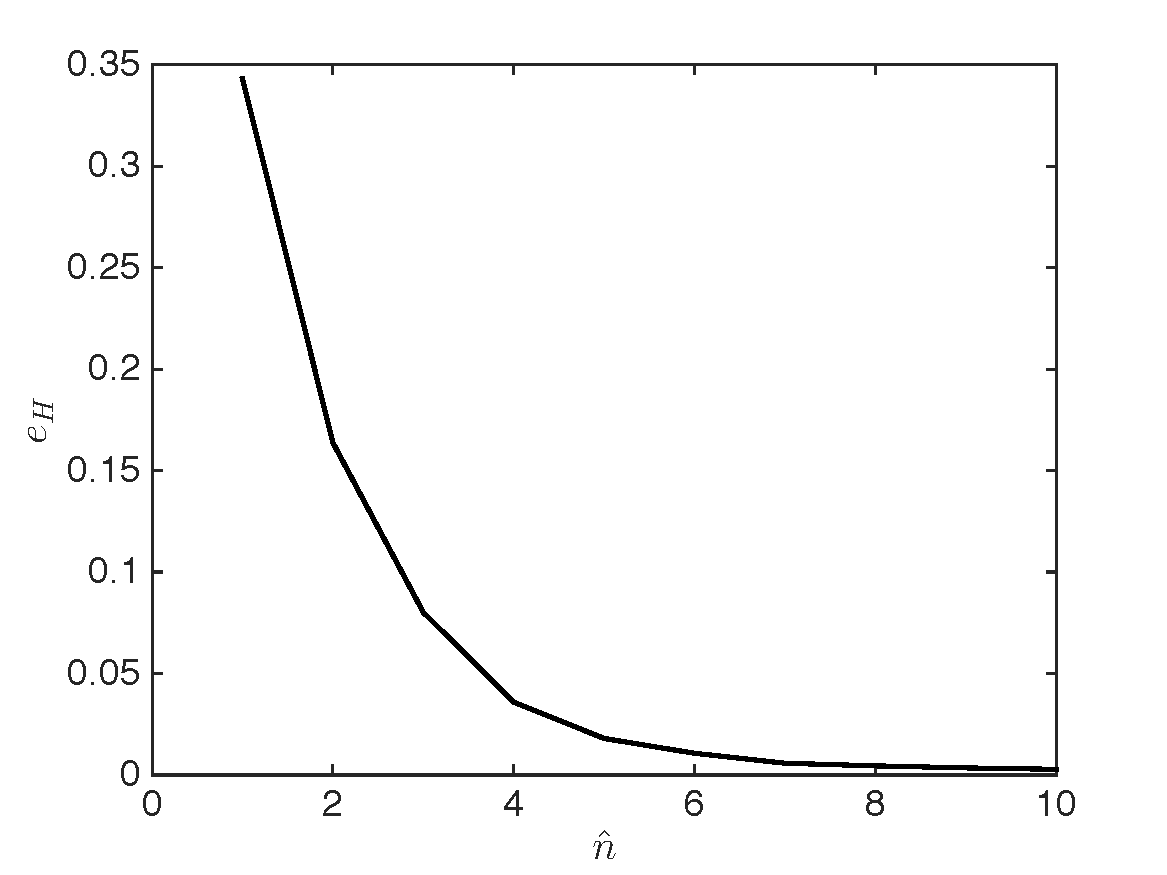
\includegraphics[width=\textwidth]{JustifyApprox_eH.pdf}
        		\caption{Entropy Error}
        		\label{fig:H_err}
    	\end{subfigure}
	\begin{subfigure}[b]{0.45\textwidth}
        		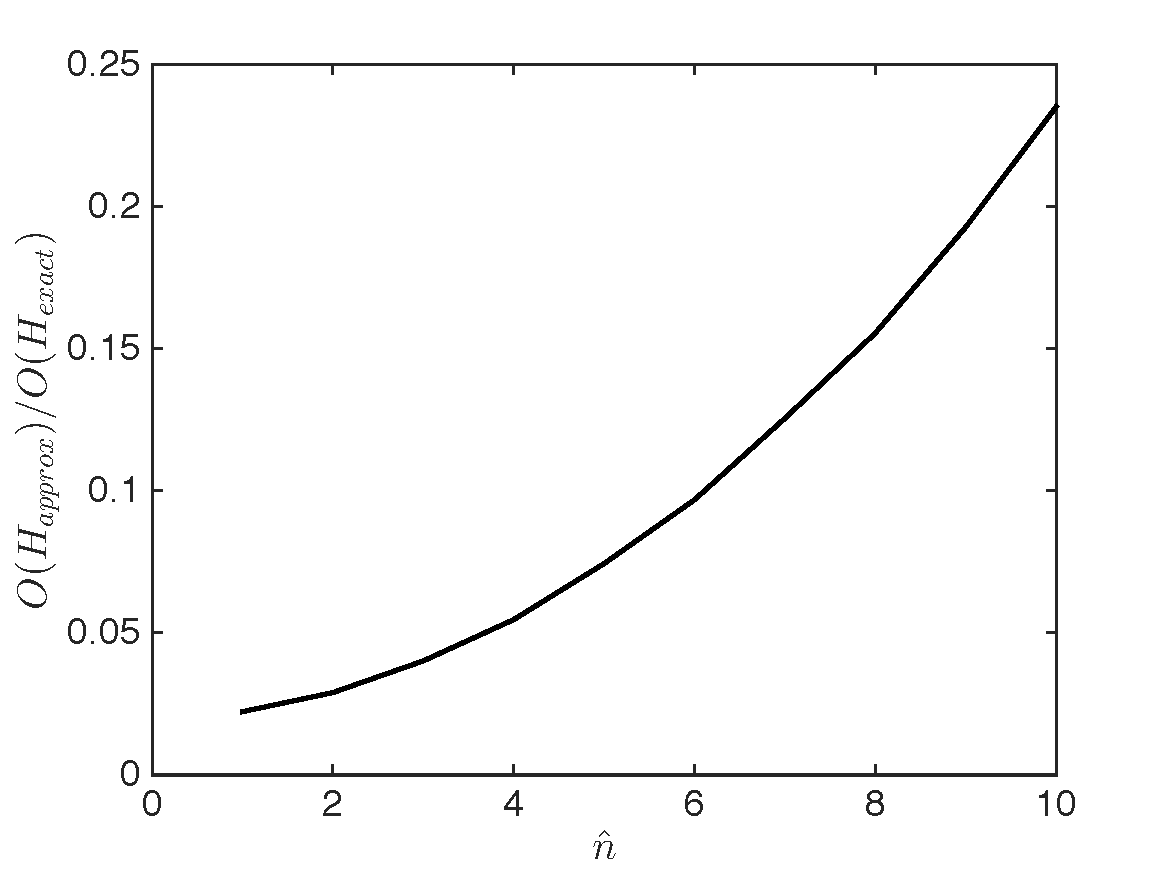
\includegraphics[width=\textwidth]{JustifyApprox_t.pdf}
        		\caption{Computation Ratio}
        		\label{fig:H_comp_ratio}
    	\end{subfigure}
\caption{The entropy error is decreased at the cost of increasing computation time in this Monte Carlo 1D measurement ray expected entropy case.}
\label{fig:ApproxJust}
\end{figure}





\section{Future Pose Optimization}

\subsection{Optimal Attitude from Sample Rays}
% SIMPAR figure on optimal pose

%Then, \refeqn{DiscExpEntropyRay} is applied repeatedly over several sample measurement rays that compose scan $Z_c$ as shown in~\cite{KauAiLee16}.

\subsection{Travel Cost with Obstacles}
% Dijkstra's cost map

\subsection{Optimal Pose Selection}
% Single-Vehicle argmax

\subsection{Collision-Free Motion Planning}
% Dijkstra's algorithm (after cost map), no least squares yet

\section{Numerical Examples}

\subsection{Exploring a Simple Environment}
% SIMPAR numerical example (2 rooms, 1 hallway)

\subsection{Exploring a Complicated Benchmark Environment}
% JINT17 Fig. 7 & 8

\section{Experimental Result}
% JINT17 9, 10, 11 (ground experiment at the NRL)

\section{Conclusions}


